%% Copyright 2023 P. S. Eduardo.
%
% This work may be distributed and/or modified under the
% conditions of the LaTeX Project Public License, either version 1.3
% of this license or (at your option) any later version.
% 
% The Current Maintainer of this work is P. S. Eduardo.
%
% This work consists of the file poli.cls.
%% -----------------------------------------------------------------
% Escola Politécnica UFRJ LaTeX Template
% Version: 2302
% Author: Eduardo Paiva dos Santos
% email: eduardopaiva@poli.ufrj.br
% Base: CoppeTeX 2.3
%%------------------------------------------------------------------
\documentclass[grad,pdftex]{poli}
\usepackage[utf8]{inputenc}
\usepackage{amsmath,amssymb}
\usepackage{amsthm}
\usepackage{float}
\usepackage{multirow}
\usepackage{longtable}
\usepackage{tikz}
\usetikzlibrary{shapes,arrows,chains,positioning,calc}
\usepackage{enumitem}
\usepackage{indentfirst}
\usepackage{array}
\usepackage{diagbox}
\usepackage{natbib}
\usepackage[english]{babel}
\selectlanguage{english}
\usepackage{subcaption}
\usepackage{listings}
%\usepackage[alf, bibjustif]{abntex2cite}
\usepackage{comment}
\makelosymbols
\makeloabbreviations
\usepackage{lineno}
\usepackage{algorithm} %primeiro pacote de algoritmo que já funciona
\usepackage{minted} %teste de um pacote que aparece em python e fica colorido
\usepackage[noend]{algpseudocode}
\linenumbers

\newtheorem{theorem}{Theorem}
\newtheorem{conjecture}[theorem]{Conjecture}
\newtheorem{lemma}[theorem]{Lemma}
\newtheorem{fact}[theorem]{Fact}
\newtheorem{proposition}[theorem]{Proposition}
\newtheorem{definition}[theorem]{Definition}
\newtheorem{corollary}[theorem]{Corollary}

\begin{document}
  \selectlanguage{english}
  \title{Título do TCC}
  \foreigntitle{TCC Title}
  \author{Rodrigo}{Mendes Palmeira}
  \advisor{Prof.}{Fábio}{Botler}{D.Sc.}
  %\coadvisor{Prof.}{Nome}{Sobrenome}{D.Sc.}
  \examiner{Prof.}{Nome Completo}{Ph.D.}
  \examiner{Prof.}{Nome Completo}{D.Sc.}
  %\examiner{Prof.}{Nome Completo}{D.Sc.}
  \department{DNC} %UTTILIZE A SIGLA DO SEU DEPARTAMENTO MODIFICAR OS NOMES DE CURSO, DEPARTAMENTO E OBTENÇÃO DE GRAU (Obs: caso tenha algum equívoco nesses argumentos, necessário modificar o arquivo poli.cls no local que faz a leitura deste argumento)
  \date{2}{2023}
  \keyword{keyword1}
  \keyword{keyword2}
  \keyword{keyword3}
  \keyword{keyword4}
  \maketitle

  \frontmatter
  \include{Pre-textual/dedic}
  \include{Pre-textual/thanks}
  \include{Pre-textual/resumo}
  \include{Pre-textual/abstract}
  \tableofcontents
  \listoffigures
  \listoftables
  \printlosymbols
  \printloabbreviations

  \mainmatter
    \chapter{Introduction}
TODO: 
Definições de grafo, grafos cúbicos,homomorfismo e profas auxiliadas por computador 

SENTENCE SUGGESTION: whenever possible, we illustrate definitions and methods with python based algorithms

\section{Graphs}

Graphs are mathematical structures first described by \emph{Euler} to solve the \emph{Seven Bridges of Königsberg} problem - TODO add citation -. 
Are used to model different gammas of real world problem including deadlock detection, shortest paths, package routing, among numerous others. 

A Graph $G$ can be defined as a set of vertices $V(G) \subset \mathbb{N}$ and edges $E(G) \subseteq [V^2]$. 
For every $\{u, v\} \in E(G)$, we call $u$ and $v$ neighbours. 
We say that the neighborhood $N_G(v)$ of a vertex $v \in V(g)$ are neighbors of $v$ in $G$ and the degree $d_G(v)$ as $|N_G(v)|$.
A graph for which the degree of every vertex has the same value $r$ is a $r$-$regular$ graph and, specifically, for $r=3$ a \emph{cubic} graph.
A \emph{complete graph} is a $(n-1)$-$regular$ graph where $n=|V(G)|$.
$K_n$ is the complete graph of size $n$.

We say that the graph $G'$ is a \emph{subgraph} of the graph $G$ if and only if $V(G') \subset V(G)$ and $E(G') \subset E(G)$, we, then, can write $G' \subset G$. 
A \emph{path} $P$ in a graph $G$ is a sequence of vertices $(x_1, \dots, x_k)$ such that, for every $1 \leq i < k$, $\{ x_i, x_{i+1} \} \in E(G)$. 
If all vertices in $P$ are distinct and $\{ x_1, x_k \} \in E(G)$, we call it a \emph{cycle} with size $k$.
$G$ is \emph{connected}, if for every pair of vertices $u$ and $v$ in $G$, there is a path starting in $u$ and ending in $v$.

TODO: [n]

$C_n$ is a graph with $n$ vertices such that there is cycle $P=(x_1, \dots, x_n)$ and $E(C_n) =\{ \{x_i,x_{i+1}\} | 1 \leq i < n \} \cup \{\{x_1,x_n\}\}$. 
It's easy to that $K_3$ and $C_3$ are the same graph show on Figure \ref{fig:k3}.
The \emph{girth} $g$ of Graph $G$ is length of the the shortest cycle which is a subgraph of $G$.
If there is no such cycle, $G$ is \emph{acyclic} with girth $g= \infty$.

We say that a graph is a \emph{tree} if it is acyclic and connected. Vertices in a tree are a called leafs nodes if their degree is one and internal otherwise.  

For any graphs $G_1$ and $G_2$, a homomorphism is a function $h \colon G_1 \to G_2$ such that $\{h(u), h(v)\} \in E(G_2)$ for every edge $\{u, v\} \in E(G_1)$. 

Given graphs \(G\) and \(H\), an \emph{homomorphism} from \(G\) to \(H\)
is a function \(h\colon V(G) \to V(H)\) for which \(h(x)h(y)\in E(H)\) whenever \(xy\in E(G)\).
For ease of notation, in this case, we write \(h\colon G \to H\).


 \begin{figure}
    \centering
    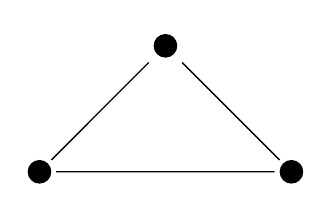
\begin{tikzpicture}[node distance=2cm,scale = .8]
% Vértices
\tikzset{black vertex/.style={circle,draw,minimum size=1mm,inner sep=0pt,outer sep=2pt,fill=black, color=black}}

  \node (0) at (0,0) {0};
  \node[black vertex] () at (0,0) {0};
  \node[black vertex] (1) at (2,-2) {1};
  \node[black vertex] (2) at (-2,-2) {2};

% \draw[line width = .5pt] (0) -- (1) (2) -- (3) (4) -- (5) (6) -- (7) (8) -- (9) (10) -- (11) (12) -- (13) (14) -- (15);

\draw[line width = .5pt] (0) -- (1) (0) -- (2) (1) -- (2) ;

\end{tikzpicture}
    \caption{$K_3$}
    \label{fig:k3}
\end{figure}



\section{Computer-assisted proofs}

    \chapter{Motivation and Initial Definitions}
\label{chap2}
\newcommand{\nesetril}{Ne{\v{s}}et{\v{r}}il}
\newcommand{\devos}{DeVos}
\newcommand{\samal}{{\v{S}}{\'a}mal}
\newcommand{\bads}{{\rm Bads  }}
\newcommand{\girth}{g}
\newcommand{\dist}{{\rm dist}}
% \newcommand{\samal}{{\v{S}}{\'a}mal} 
\newcommand{\cleb}{Clebsch graph}

\newcommand{\cost}{{\rm cost}}
%
% \section{TODOS}
% \begin{itemize}
% % \item Testar com o seguinte grafo de Clebsch modificado ao adicionarmos todas as arestas incidentes ao 0.
% % \item Testar nível 4 com quadruplas 
% % \item Remover referência a super grafo 
% % \item Testar todas as quadruplas e calcular números de raizes possíveis 
% % \item Adpatar a parte de replacements para Clebsch novamente e falar dos triviais 
%
% \item Prova de conceito
% \item Na seção de resultados falar que a técnica funciona pro supergrafo de Clebsch. Infelizmente, há um homomorfismo trivial para este grafo.
%
% \item Que condições a gente precisa pra essa estratégia funcionar? (1) que qualquer par de vértices com distância 2 tenha pelo menos dois vizinhos em comum.
%
% \item Perspectiva geral: recebemos um grafo cúbico que admite um homomorfismo a um grafo H, será que conseguimos evitar algum vértice adicionando uma condição na cintura de G?
%
% \end{itemize}

In what follows, if \(m\) is a function \(m\colon A \to B\) and \(A'\subseteq A\),
we denote by \(m|_{A'}\) the restriction of \(m\) to \(A'\),
i.e., the function \(m|_{A'}\colon A' \to B\)
such that \(m|_{A'}(x) = m(x)\) for every \(x\in A'\).

Let \(T\) be a tree in a cubic graph \(G\).
A vertex \(x\) such that \(d_T(x) = 1\) is called a \emph{leaf} of \(T\),
otherwise \(x\) is called \emph{internal}.
We say that \(T\) is \emph{cubic} if \(d_T(x)\in\{1,3\}\) for every vertex of \(T\).

%TODO talvez queiramos isso para sequências de vértices.
%TODO verificar se usamos apenas o conjunto de cores
% Let $h$ be any homomorphism $h \colon G \to G'$ and $T \subseteq G$ a tree, we define $h(L(T))$ as the set $\{ h(x) : x \in L(T)\}$.

Let $h$ be a homomorphism $h \colon G \to G'$ and let \(S\) be a tuple \((u_1,\ldots,u_s)\) of vertices of a graph.
Denote the tuple \(\big(h(u_1),\ldots, h(u_s)\big)\) as $h(s)$.

Given a complete tree $T$ of height \(h\geq 1\), the \emph{internal induced subtree} $T^{(1)}$ is the subtree of \(T\) induced by the vertices in $V(T) \setminus L(T)$. 
Additionally, we define $T^{(2)}$ to be $(T^{(1)})^{(1)}$ and, 
more generally, if \(d < h\), then $T^{(d)} = (T^{(d-1)})^{(1)}$.


\subsection{The Clebsch graph}\label{sec:clebsch}
The Clebsch graph (see Figure~\ref{fig:clebsch_graph}) is the $5$-regular graph \(CH = (V_1 \cup V_2 \cup V_3, E)\), where
$V_1 = \big\{ \{x\} : \text{ for all } x \in [5] \big\}$, $V_2= \big\{ \{x,y\} : \text{ for all } x, y \in [5] \text{ such that } x < y \big\}$, $V_3 = \big\{ \{ 1,2,3,4,5 \} \big\}$ and
\[E = \big\{ XY : X \in V_1,\ Y \in V_2\cup V_3\text{ and } X \subseteq Y\big\} \cup \big\{ XY : X,\ Y \in V_2,\ X \cap Y = \emptyset  \big\}.\]

Throughout the text we refer to the vertices of \(\ch\) as $0, \ldots, 15$ as show in Figure~\ref{fig:clebsch_graph} 
and, to avoid confusion with the vertices of the studied cubic graphs, we refer to the vertices of \(\ch\) as \emph{colors}.
Moreover, we often refer to homomorphims to $\ch$ as colorings.
A key observation with respect to \(\ch\) that is used throughout the text is that every pair of (not necessarily distinct) colors has either zero, two, or five common neighbors.
\begin{fact}\label{fact:common_neighbors}
    If \(u,v \in V(\ch)\), then \(|N(u)\cap N(v)| \in \{0,2,5\}\).
\end{fact}

\section{The Pentagon Problem}
\label{sec:the-pentagon-problem}

This work concerns about the \emph{\nesetril{} Pentagon Problem} stated below. 

% já definiu homorphism?
% já definiu o C5?
% Já definiu cubic graph?
% já definiu cintura?
\begin{conjecture}\label{conj:pentagon-problem}
    There is a constant \(g_0\in \mathbb{N}\) for which the following holds.
    If \(G\) is a cubic graph with girth at least \(g_0\),
    then \(G\) has a homomorphism to $C_5$.
\end{conjecture}

Conjecture~\ref{conj:pentagon-problem} was originally proposed in \nesetril{} problem sessions~(see \cite{nesetril1999aspects}). 
By Brook's Theorem (see~\cite{Brooks1941} or~\cite[Theorem 5.2.4]{diestel2017graph}),
every triangle-free cubic graph has chromatic number at most \(3\),
and hence is homomorphic to \(C_3\).
On the other hand, \cite{HATAMI2005319} showed that Conjecture~\ref{conj:pentagon-problem} does not hold 
if we replace \(C_5\) by \(C_\ell\) for any \(\ell>5\),
i.e., that for every \(\ell\) and \(g\) there is a cubic graph of girth at least \(g\) that is not homomorphic to \(C_\ell\).
Conjecture~\ref{conj:pentagon-problem} deals then with the remaining case of \(C_5\).

\begin{figure}[h]
     \begin{subfigure}[b]{0.45\textwidth}
         \centering
         \input{Imagens/C5}
         \caption{The cycle $C_5$ of length $5$}
         \label{fig:c5}
     \end{subfigure}
     \begin{subfigure}[b]{0.45\textwidth}
         \centering
         \input{Imagens/clebsch_graph}
         \caption{The Clebsch Graph $\ch$}
         \label{fig:clebsch_graph}
     \end{subfigure}
     % \caption{Left: the cycle $C_5$ of length $5$; Right: The Clebsch Graph $\ch$}
     \caption{}
     \label{}
\end{figure}

\newcommand{\ch}{{CH}} 
\newcommand{\chzero}{{CH_0}}
\newcommand{\chone}{{CH_1}}
As an approximate result, in a computer-assisted proof, \cite{devos2011high} showed that every graph $G$ with $\Delta(G) \leq 3 $ and girth at least 17 has a homomorphism to the \emph{Clebsch graph}
that can be computed by a liner time algorithm.

\begin{theorem}[\devos--\samal]\label{thm:DevosSamal11}
Every graph of maximum degree 3 and girth at least 17 is homomorphic to $\ch$.
\end{theorem}

%TODO: falar que "It is then natural to consider other computer search methods in order to improve Theorem 2"

% TODO falar em algum lugar da transitividade dos homomorfismos: se G -> H e H-> R, então G -> R

% Observe ao removermos os vértices \(0,1,2,7,12\) do grafo de Clebsch, obtemos um grafo que admite um homomorfismo para o \(C_5\).
% Assim, se há um homomorfismo de \(G\) ao grafo de Clebsch que evita tais vértices, há um homomorfismo de G para C_5.
% Em particular, sejam V1,...,V5 as classes de um homomorfismo h^-: C^- = Clebsch-{0,1,2,7,12} -> C5, tais que os vértices de V_i são adjacentes apenas aos vértices de V_{i-1} e V_{i+1}, onde a soma nos índices é tomada módulo 5.
% 
We consider the possibility of building upon Theorem~\ref{thm:DevosSamal11} to get a stronger result towards Conjecture~\ref{conj:pentagon-problem} using the following simple observation:
there is a small set \(B\subseteq V(\ch)\) such that the graph obtained from \(\ch\) by removing the vertices in \(B\)
is homomorphic to \(C_5\).
Although there are several sets with the property above, in this work we use the set \(B_0 = \{0,1,2,7,12\}\),
which we call the set of \emph{undesired colors},
and we denote by \(\ch_0\) the graph obtained from \(\ch\) by removing the vertices in \(B_0\).
It's not hard to check that \(CH_0\) has a homomorphism \(h_0\) to $C_5$\footnote{For example pick the graph classes \{4, 8\}, \{9,10,14\}, \{6,11,15\}, \{3, 13\}, \{5\}},
and hence, to solve Conjecture~\ref{conj:pentagon-problem}, it's enough to prove that there is a constant \(g_0\) for which every cubic graph with girth at least \(g_0\) has a homomorphism to \(CH_0\),
i.e., a homomorphism to \(CH\) that avoids the vertices in \(B_0\).
%
The objective of this work is to explore computer assisted methods to 
find a partial result in this direction.
More specifically we want to find a minimum girth \(g_0\)
for which all cubic graphs of girth at least $g_0$ have a homomorphism to 
the graph \(\chone\) obtained from \(\ch\) by removing a non-empty subset $B_1 \subseteq B_0$. 


We establish a theoretical framework for locally recoloring the extended neighborhood of a vertex, that, due to the high girth condition, is isomorphic to a tree, 
in order to avoid undesired colors.
We use this framework to prove the trivial result that we can always remove one of the undesired vertices from any homomorphism from a cubic graph of girth at least $17$ to a degenerate form of Clebsch graph that contains a few triangles. Furthermore, we try unsuccessfully to use it to remove a color from any homomorphism from a cubic graph of girth at least $g$ to the Clebsch graph,
and present some statistical results regarding the number of \emph{configurations} (see Section~\ref{sec:configurations})
that can be ``improved'' using this method.
On the other hand, we present an infinite family of configurations that, independently of the girth, cannot be locally improved (see Chapter~\ref{chap5}).
This proves the non-effectiveness of this method.

The main contribution of this work is the theoretical foundation that enables this framework which
can be further used to explore different subgraphs (See Chapter~\ref{chap6})
as cycles, for which it is still not clear if the above intrinsically bad configurations also provide obstructions.

\section{Theoretical foundation}\label{sec:theoretical-foundation}

In order to avoid undesired colors, we need to 

Let \(G\) be a subcubic graph, and let \(h\) be a homomorphism $G \to \CH$.
We define the \emph{cost} of $h$ as 
\[\cost(h)~=~|\{x : \text{ for all } x \in V(G) \text{ and } h(x) \in B_1 \}|.\] 

Observe that, if \(\cost(h) = 0\), then \(h\) avoids the vertices in \(B_1\),
and hence, as observed in Section~\ref{sec:the-pentagon-problem},
\(h\) is a homomorphism from $G$ to $\chone$.


Now, let \(G\) be a cubic graph,
let \(T\subseteq G\) be a cubic tree,
and suppose that exists a homomorphism \(h \colon G \to \ch\).
We say that a homomorphism \(h' \colon T \to \ch\) is \(h\)-\emph{compatible} if \(h'|_{L(T)} = h|_{L(T)}\),
i.e., if \(h'(x) = h(x)\) for every \(x\in L(T)\),
and we define the \((h,h')\)-\emph{modified} map $h^* \colon G \to \ch$ by
\[ 
h^*(v) = 
     \begin{cases}
       h'(v) &\quad\text{if } v\in V(T)\\
       h(v) &\quad\text{if } v\notin V(T).
     \end{cases}
\]

By the definition of \(h\)-compatible, 
if \(d_T(u) = d_G(u)\) for every vertex of \(T\) that is not a leaf, 
then $h^*$ is a homomorphism from \(G\) to \(CH\).
Indeed, let \(uv\in E(G)\). 
If \(uv\in E(T)\), then \(h'(u)h'(v) \in E(CH)\) because \(h'\) is a homomorphism from \(T\) to \(CH\).
Now, suppose that \(uv\notin E(T)\).
If both $u$ and $v$ are in $V(G) \setminus V(T)$ we have $h^*(u)h^*(v) = h(u)h(v)$ which in $E(CH)$ because \(h\) is is a homomorphism from \(G\) to \(CH\).
If $u \in V(T)$ and $v \in V(G) \setminus V(T)$, then $u$ is a leaf of $T$.
By the definition of \(h\)-compatible we have $h'(u) = h(u)$ and hence $h^*(u)h^*(v) = h(u)h(v)$ which is in \(E(CH)\) because \(h\) is is a homomorphism from \(G\) to \(CH\).

%Definição alternativa de custo
%Now, let \(G'\) be a subgraph of \(G\), 
%and let \(m\colon V(G')\to V(H)\).
%We define the \(\cost(m)\) as the number of elements of \(V(G')\) mapped to $0$,
%i.e., the size of \(\{x\in V(G') : m(x) = 0\}\).
The following lemma comes naturally.

\begin{lemma}\label{lemma:cost-improvement}
    Let \(G\) be a cubic graph for which there is a homomorphism \(h\) from \(G\) to \(CH\), let $T \subseteq G$ a cubic tree, $h'$ a $h$-compatible homomorphism from $T$ to $\ch$,
    and let \(h^*\) be the \((h,h')\)-modified homomorphism,
    then \[\cost(h^*) = \cost(h) - \cost(h|_T) + \cost(h').\]
\end{lemma}

% Similarly, if both $u$ and $v$ are in $G \setminus T$ we have $(h_1(u), h_1(v)) = (c(u), c(v)) $ which by definition is in $E(H)$. If $u \in T$ and $v \in G \setminus T$ we have that necessarily u is a leaf of $T$ and therefore, by the definition of \(c\)-\(\compatible\), $ c_2(u) = c(u)$ and $(h_1(u), h_1(v)) = (c(u), c(v)) $ which by definition is in $E(H)$. 
% We also have that : 
%%%USAR ALIGN AQUI
% $$
% cost(h_1) = | \{x\in V(G) : h_1(x)\in\bads\} | 
% $$
% \[= | \{x\in V(G \setminus T) : c(x)\in\bads\} | + | \{x\in V(T) : c_2(x)\in\bads\} | \]
% \[= | \{x\in V(G) : c(x)\in\bads\} | -  |\{x\in V(T) : c(x)\in\bads\} | + cost(c_2) \]
% \[= cost(c) - | \{x\in V( T) : c(x)\in\bads\} | + cost(c_2) \]
% \[= cost(c) - cost(c|_T) + cost(c_2) \]
\begin{proof}
    \begin{align*}
    \cost(h^*) 
        & = | \{x\in V(G) : h^*(x)\in\bads\} | \\
        & = | \{x\in V(G) \setminus V(T)) : h(x)\in\bads\} | + | \{x\in V(T) : h'(x)\in\bads\} | \\
        & = | \{x\in V(G) : h(x)\in\bads\} | -  |\{x\in V(T) : h(x)\in\bads\} | + cost(h') \\
        & = \cost(h) - | \{x\in V( T) : h(x)\in\bads\} | + cost(h') \\
        & = \cost(h) - \cost(h|_T) + \cost(h') \qedhere.
    \end{align*}
\end{proof}

Now, suppose that \(h\) is a homomorphism from \(G\) to \(\ch\) 
that minimizes \(\cost(h)\).
Let \(T\subseteq G\) be a cubic tree,
and let \(h'\) be a \(h\)-compatible homomorphism of \(T\).
%
Consider the \((h,h')\)-modified homomorphism \(h^*\).
If \(\cost(h') < \cost(h|_T)\), then \(h^*\)
is a homomorphism of \(G\) in \(\CH\) for which, by Lemma~\ref{lemma:cost-improvement}, we have \[\cost(h^*) = \cost(h) - \cost(h|_T) + \cost(h') < \cost(h),\]
a contradiction to the minimality of \(h\).
Therefore, for every cubic tree \(T\subseteq G\) there is no \(h\)-compatible homomorphism \(h'\) of \(T\) for which \(\cost(h') < \cost(h|_T)\).
This yields the following lemma

\begin{lemma}\label{lemma:there-is-no-improvement}
Let \(G\) be a cubic graph with girth at least \(\girth{}\),
and let \(h\) be a homomorphism from \(G\) to \(CH\) 
that minimizes \(\cost(h)\).
Now, let \(T\subseteq G\) be a cubic tree. 
Then there is no \(h\)-compatible homomorphism \(h'\colon T \to CH\)
such that \(\cost(h') < \cost(h|_T)\).
\end{lemma}

The methods developed in this work mean to explore the following conjecture.

\begin{conjecture}\label{conj:main-conjecture}
Let \(G\) be a cubic graph with girth at least \(\girth{}\) for which there is a homomorphism \(h\) from \(G\) to \(CH\).
If \(\cost(h) > 0\),
then there is a cubic tree \(T\subseteq G\)
and a \(h\)-compatible homomorphism \(h'\) from \(T\) to \(CH\)
such that \(\cost(h') < \cost(h|_T)\).
\end{conjecture}

If Conjecture~\ref{conj:main-conjecture} holds,
then if \(h\) is a homomorphism from \(G\) to \(CH\) 
that minimizes \(\cost(h)\),
then \(\cost(h) = 0\).
Therefore, as a natural consequence of Lemma~\ref{lemma:cost-improvement} and Conjecture~\ref{conj:main-conjecture}, we have the following.

%TODO: revisar isso quando checar se a prova funciona para H no lugar de H^+
\begin{theorem}\label{thm:main}
    % Suppose that Conjecture~\ref{conj:main-conjecture} holds.
    % If \(G\) is a cubic graph of girth at least \(\girth\),
    % then there is a homomorphism from $G\to CH_1$.
% 
    If Conjecture~\ref{conj:main-conjecture} holds,
    then every cubic graphs with girth at least \(\girth\) has a homomorphism to \(\chone\).
\end{theorem}

\begin{proof}
Let \(G\) be as in the statement.
By Theorem~\ref{thm:DevosSamal11}, there is a homomorphism from \(G\) to \(CH\).
Let \(h\) be a homomorphism from \(G\) to \(CH\) that minimizes \(\cost(h)\).
Suppose \(\cost(h) > 0\). 
If Conjecture~\ref{conj:main-conjecture} holds, then there is a cubic tree \(T\subseteq G\)
and a \(h\)-compatible homomorphism \(h'\) from \(T\) to \(CH\)
such that \(\cost(h') < \cost(h|_T)\).
Now, let \(h^*\) be the \((h,h')\)-modified homomorphism from \(G\) to \(CH\).
By Lemma~\ref{lemma:cost-improvement}, we have \(\cost(h^*) = \cost(h) - \cost(h|_T) + \cost(h') < \cost(h)\),
a contradiction to the choice of \(h\).
Therefore, we have \(\cost(h) = 0\), and hence \(h\) is a homomorphism from \(G\) to \(\chone\) as desired.
\end{proof}


    
    \chapter{Classifying Configurations}
\label{chapter:implementation}

TODO: Verificar feasible capitulos anteriores
TODO: Apresentar otimizacao de utilizar good calculadas no checador de solvables 
TODO: Verificar se há parêntese colados em palavras de forma inadequada

The main strategy of this work is to explore a brute force search algorithm to determine the number of unsolvable bad configurations (see Section~\ref{sec:configurations}) of a given tree 
aiming to prove that in every tree with a given (sufficiently large) height every configuration is either good or solvable bad,
i.e., there is no bad unsolvable configuration.
In this chapter, we start with a simple version of this algorithm, discuss its complexity and limitations and then present some optimizations we used to arrive on a improved version. 
We use a python inspired pseudo-code for ease of reading (and also because we implemented a checker in Sage math see Chapter~\ref{chap:4}) and in the next chapter we present the results obtained using a \texttt{C++} version of the improved algorithm.

\section{A Simple Algorithm}\label{sec:naive-algo}
Given a tree $T$,
recall that, when \(T\) has height at least \(1\), 
\(T^{(1)}\) is the tree obtained from \(T\) by removing \(L(T)\) (See section~\ref{sec:configurations}).
By Lemma~\ref{lemma:child-costs}, we can obtain all bad configurations of \(T\) based on the costs ($RC$ and $FC$, see Definition~\ref{def:conf-costs}) of the configurations of $T^{(1)}$. 
Calculating the costs of any configuration of a tree with height $0$ is trivial and follows directly from Definition~\ref{def:conf-costs}. 
Then, to calculate the costs of any configuration \(conf\) of a tree with larger height
we can use a ``bottom-up'' recursive algorithm that 
computes these costs using the costs of each parents configuration of \(conf\) (see Algorithm~\ref{alg:naive-bottom-up:costs}).

\begin{algorithm}
\caption{Naive algorithm for calculating costs using a ``bottom-up'' strategy}\label{alg:naive-bottom-up:costs}
\footnotesize
\begin{minted}[xleftmargin=\parindent,linenos, breaklines, escapeinside=||,mathescape=true]{python}
def CalculateCosts(T, conf):
    if len(conf) == 1:
        if(conf[0] in |$B_1$|):
            return 1,1
        else:
            return 0, |$\infty$|
    #respectively the min parent free cost and the min parent restricted cost
    minpfc, minprc = |$\infty$|, |$\infty$| 
    levelcost    = sum([1 for x in conf if x in |$B_1$|])
    for confp in ParentConfigurations(T,conf):
        pfc, prc  = CalculateCosts(|$T^{(1)}$|, confp)
        minpfc, minprc = min(minpfc, pfc), min(minprc, prc)
    return minpfc + levelcost, minprc + levelcost
\end{minted}
\end{algorithm}


Note that Algorithm~\ref{alg:naive-bottom-up:costs} calls an auxiliary function \texttt{ParentConfigurations}
which returns (an iterator over) all of the parents configurations of \(conf\).
The configurations are represented as vectors of colors (integers from 0 to 15)
ordered according to their corresponding leafs which are ordered from left to right
(the orderings of the leafs are discussed more deeply in Section~\ref{sec:signatures}).

We generate the parents configurations of a given configuration $conf$ of a tree $T$ as follows.
First, note that each parents configuration is a configuration of \(L(T^{(1)})\)
such that each leaf \(\texttt{l}\) in \(L(T^{(1)})\) has a color adjacent to the colors of its children,
i.e., \(\texttt{l}\) must receive a color that is in the intersection of the neighborhoods (in $CH$)
of the colors of its children.
This results in a set of possible colors that each vertex in $L(T^{(1)})$ can be colored with. 
Then the Cartesian product\footnote{In Python the Cartesian product can be performed using the function \texttt{product} of the library \texttt{itertools}~\cite{itertools}} of these possible colors contains the set of all parents configurations of $conf$ (see Algorithm~\ref{alg:naive-bottom-up:parents}).
Note that some of those configurations may be unfeasible as it is possible to choose colors for sibling vertices in $T^{(1)}$ such that the resulting configuration cannot be completed.
The parents configurations of \(conf\)
are precisely the feasible configurations in the Cartesian product of the possible colors.
%TODO add "https://docs.python.org/3/library/itertools.html#itertools.product" no bib 

\begin{algorithm}
\caption{Returns iterator over parents configurations}\label{alg:naive-bottom-up:parents}
\footnotesize
\begin{minted}[xleftmargin=\parindent,linenos,escapeinside=||,mathescape=true]{python}
def ParentConfigurations(T, conf):
    if len(conf) == 1:
        return []
    choices = []
    for l in L(|$T^{(1)}$|):
        children    = Children(l)
        choices_p   = |$\bigcap_{i \in children} N_{CH}(conf [i] )$|
        if(len(choices_p) == 0): #guarantees earlier that conf is unfeasible
            return []   
        choices.append(choices_p) 
    return product(choices)
\end{minted}
\end{algorithm}


Finally, Algorithm \ref{alg:naive-bottom-up} returns all bad configurations on a given tree $T$ using Algorithm~\ref{alg:naive-bottom-up:costs}. 
% It generates all configurations with \texttt{product} so that we iterate over all $16^{|L(T)|}$ configurations, including the non feasible ones, and calculate its costs. 
% Calculate the costs of any given $conf$, on the other hand, iterates over all $16^{\frac{|L(T)|}{2}}$ parents configurations including non feasible ones and it calls itself recursively until the root of tree(base case) is reached. 

\begin{algorithm}
\caption{Returns all bad configurations on a given tree $T$}\label{alg:naive-bottom-up}
\footnotesize
\begin{minted}[xleftmargin=\parindent,linenos,escapeinside=||,mathescape=true]{python}
def GenerateBadConfs(T):
    bads = []
    for conf in product(list(range(0,16)), repeat = len(L(T))):
        fc, rc = CalculateCosts(T, conf)
        if(fc != |$\infty$| and fc == rc): 
            # fc != |$\infty$| means that conf is feasible
            # fc == rc means that conf is bad
            bads.Append(conf)
    return bads 
\end{minted}
\end{algorithm}

\subsubsection{Replacements}

With Algorithm \ref{alg:naive-bottom-up} we are able to determine the number of bad configurations of any given complete cubic tree. 
If there are no bad configurations, then Conjecture~\ref{conjecture:main-conjecture} is verified. 
Unfortunately, due to the exponential complexity of Algorithm~\ref{alg:naive-bottom-up},
this task cannot be pursued for a sufficiently large height.
However, by Lemma~\ref{lemma:every-good-and-solvable-configuration}, 
to prove Conjecture~\ref{conjecture:main-conjecture} it suffices to show that any complete cubic tree $T$ has no \emph{unsolvable} bad configurations. 

For this, we introduce Algorithm \ref{alg:naive-replacements} to check which of the bad configurations are solvable and, as a consequence, which are unsolvable.
% Suppose we have a set of unchecked bad configurations.
Algorithm \ref{alg:naive-replacements} checks whether, for each bad configuration that was not yet ruled out as solvable, there is a vertex $v$ colored with $c_0$ for which there is replacement $(c_0, C)$ (See Algorithm~\ref{alg:naive-replacements:check}), 
such that each similar configuration obtained by coloring $v$ with a color in $C$ is good or already know to be solvable. 

Then, on Algorithm~\ref{alg:naive-cojecture-holds}, we are able to verify if there no unsolvable bad configurations on given a complete cubic tree
by calling iteratively Algorithm~\ref{alg:naive-replacements} passing the new solvable configurations found on the previous step together with the previous already know solvables.
The algorithm stops 
when there aren't any unsolvable bad configuration left, or
when no more solvable configurations are found, since, in this case, any new call to Algorithm~\ref{alg:naive-replacements} produces the same result as there are no new know solvable configurations.

\begin{algorithm}
\caption{ClassifySolvable}\label{alg:naive-replacements}
\footnotesize
\begin{minted}[xleftmargin=\parindent,linenos,escapeinside=||,mathescape=true]{python}
def ClassifySolvable(T, bads, knownSolvablesOrGood):
    replacementsCandidates = []
    for badConf in bads: 
        for i in range(len(badConf)):
            color = badConf[i]
            siblingColor = GetSiblingColor(badConf,i) 
            newColorsToTest = CH.vertices() - CH.neighbors(siblingColor) - [color] - |$B_1$|
            C = []
            for newColorToTest in newColorsToTest:
                badConf[i] = newColorToTest
                if(badConf in knownSolvablesOrGood):
                    C.append(newColorToTest)
                    continue
                fc, rc  = CalculateCosts(T, badConf)
                if(fc != |$\infty$| and fc < rc):
                    C.append(newColorToTest)
            badConf[i] = color
            if(len(C) != 0):
                replacementsCandidates.append((badConf, i, C))
    solvableBads, unsolvableBads = [], []
    for (badConf, i, C) in replacementsCandidates: 
        if(CheckReplacement(badConf[i], C)):
            solvableBads.append(badConf)
        else:
            unsolvableBads.append(badConf)
    return solvableBads, unsolvableBads
\end{minted}
\end{algorithm}


TODO: Mover para definicao no capitulo 2 !
\begin{algorithm}
\caption{CheckReplacement}\label{alg:naive-replacements:check}
\footnotesize
\begin{minted}[xleftmargin=\parindent,linenos,escapeinside=||,mathescape=true]{python}
def CheckReplacement(c_0, C, maxLevel=3):
    T = CreateTreeForLevel(level)
    for conf in product(list(range(0,16)), repeat = pow(2, maxLevel)):
        minimalc_0Cost = MinCostWithRoots(T, conf, c_0)
        if(minimalc_0Cost == |$\infty$|):
           continue  
        if(minimalc_0Cost < MinCostWithRoots(T, conf, C)):
            return False 
    return True

def MinCostWithRoots(T, conf, possibleRoots):
    if len(conf) == 1:
        if(conf[0] in possibleRoots):
            return 0
        else:
            return |$\infty$|
    mincost = |$\infty$|
    for confp in ParentConfigurations(T, conf):
        pcost = MinCostWithRoots(T, confp, possibleRoots)
        mincost = min(mincost, pcost)
    return mincost + sum([i for c in conf if c in |$B_1$|])
\end{minted}
\end{algorithm}

\begin{algorithm}
\caption{ConjectureHolds}\label{alg:naive-cojecture-holds}
\footnotesize
\begin{minted}[xleftmargin=\parindent,linenos, breaklines, escapeinside=||,mathescape=true]{python}
def ConjectureHolds(T):
    unsolvedBads = GenerateBadConfs(T)
    knownSolvables = []
    while(unsolvedBads > 0):
        newSolvableBads, newUnsolvedBads = ClassifySolvable(T, unsolvedBads, knownSolvables)
        if(len(newUnsolvedBads) == len(unsolvedBads)):
            break
        unsolvedBads = newUnsolvedBads 
        knownSolvables.extend(newSolvableBads)
    return unsolvedBads == 0
\end{minted}
\end{algorithm}

\subsubsection{Complexity}


The algorithm described in this chapter has clearly an exponential behavior.
Thus, for completeness, we present a brief complexity analysis of its worst-case scenario.
This analysis also motivates the optimizations presented in Section~\ref{sec:signatures}. 
The algorithm traverses all the $16 ^{|L(T)|}$ possible configurations of $T$.
For each such configuration, it calls CalculateCosts which calls it self recursively for each of its parents configurations. 
Each father can be colored with at most five colors (this happens when all children are colored with the same color),
and hence the number of parents configurations is at most \(5^p\),
where \(p\) is the number of parents (which vary corresponding to the level of the tree).
% It finds the parents configurations by seeing, for each sibling pair or triple on the root's children, which colors can color the leaf's parents such that it is adjacent to all colors of its children.
% In the binary case, we have 3 distinct possibilities: 5 colors if both siblings are colored the same(recall that \ch~is 5-regular), 2 if the siblings are colored withall non distinct non adjacent colors and 0 on the remaining case. 
% In the root case, all possibilities remain and there is also the case of only one color choice for the root. 
% Therefore CalculateCosts calls it self $O(5^{\frac{L(T)}{2}})$ times.
Therefore in the worst-case scenario, the number of steps performed is at most \[16^{|L(T)|}\cdot 5^{\frac{|L(T)|}{2}}\cdot 5^{\frac{|L(T)|}{4}} \cdot \cdots \cdot 1\leq \big(16 \cdot 5^{\frac{1}{2} + \frac{1}{4} + \cdots } \big)^{|L(T)|} \leq 80^{|L(T)|}.\]

\section{Signatures}\label{sec:signatures}
First, in order to reduce the computer effort of testing all such configurations, we present one of the optimizations we used. 
More precisely, we define the \emph{signature} of a configuration,
which defines equivalence classes between the configurations.

\newcommand{\p}{{\rm p}}
Let \(T\) be a complete tree rooted on a vertex \(r\).
We say that a vertex \(v\) is a \emph{child} of a vertex \(u\)
if \(v\) is a neighbor of \(u\) that is not in the (unique) path from \(u\) to \(r\).
Equivalently, we say that \(u\) is the \emph{father} of \(v\),
and we write \(\p(v)\) for the father of a vertex \(v \neq r\),
and \(children(u)\) for the set of children of \(u\).
In this work, we consider orderings \(children(u)\),
and we write \(children(u) = (x_1,\dots,x_n)\) as an ordered set.
Given such an ordering
\(children(u) = (x_1,\dots,x_n)\), we write \(x_{i} < x_{i+1}\) for all $1 \leq i < n$.
Note that the union of these orders over the set of vertices of~\(T\)
yields a partial order of the vertices of \(T\).
Such a union of orderings is called \emph{children ordering}.
This order can be naturally extended to a total order of each level of the tree by setting that if \(u < v\), then \(x < y\) for every \(x\in children(u)\) and \(y\in children(v)\),
and this consequently yields a total order of the leaves of \(T\).


% Observe that, by definition, if \(v\in L(T)\), 
% then $ldf(v)~=~\{v\}$.
% Equivalently, \(ldf(v)\) consists of the leaves of the (tree) component of \(T-vv^p\) that contains~\(v\).
% %
% % Given an internal vertex \(v\),
% % let \(v^p\) be the vertex for which \(v\in children(v^p)\).
% % We define the \emph{leaves of} \(v\)
% % as the leaves of the (tree) component of \(T-vv^p\) that contains~\(v\).
% In the case \(v = r\), we have \(ldf(v) = L(T)\).
% We also assume that the \(ldf(v)\) inherit the total order of \(L(T)\) for every \(v\in V(T)\).

% Now, let \(x_1,\ldots, x_\ell\) be the leaves of \(T\)
% ordered as above.
% Let $V_\ell$ be the vertices at distance $\ell$ of $r$,
% the \emph{descendant leaves} of a vertex $v$ be all leafs of $T$ with $v$ within it's unique path to $r$,
% \(conf\) a feasible configuration on \(T\),
% and fix a children ordering~\(o\).
% We consider a coloring \(c_o\) of the internal vertices of \(T\) with sequences of colors as follows.
% Let \(x\in V(T) \setminus L(T)\) an internal vertex, and let \(y_1,\ldots, y_k\) be the (ordered) descendant leaves of \(x\).
% We then set \(c_o(x) = \big(conf(y_1),\ldots,conf(y_k)\big)\).
% % Such a coloring \(c_o\) is called the \emph{ordered coloring} of \(x\) 
% % induced by \(conf\).
% Observe that if \(T\) has height \(\ell\),
% and \(x\in V_s\), then \(c_o(x) \in V(CH)^{\ell - s}\).
% Consequently, if \(r\) is the root of \(T\),
% then \(c_o(r) \in V(CH)^\ell\).

\newcommand{\sign}{{\rm sign}}

Now, fix a children ordering \(o\).
We consider a partial order on sequences of colors as follows.
Let \(u, v, w\in V(T)\) be such that \(v, w \in children(u)\).
If \(v\) and \(w\) are leaves of \(T\), 
then we write \(c_o(v) < c_o(w)\) if \(conf(v) < conf(w)\) and \(c_o(v) \geq c_o(w)\) otherwise.
If \(v\) and \(w\) are internal vertices of \(T\),
with \(children(v) = (x_1, \dots, x_n)\) and \(children(w) = (y_1,\dots,y_n)\),
then we write \(c_o(v) < c_o(w)\) 
if for the minimum \(i\) with $1\leq i \leq n$ such that $c_o(x_i) \neq c_o(y_i)$, we have \(c_o(x_i) < c_o(y_i)\);
and $c_o(v) = c_o(w)$ if for every $i$ with $1\leq i \leq n$ we have \(c_o(x_i) = c_o(y_i)\);
and \(c_o(v) > c_o(w)\) otherwise.
Then \(\leq\) and \(\geq\) are defined as usual.
% This ordering is a recursive lexicographic ordering.
% Naturally, we write \(c_o(v) = c_o(w)\) if \(c_o(x_1) = c_o(y_1)\) and \(c_o(x_2) = c_o(y_2)\),
% and we write \(c_o(v) \leq c_o(w)\) if either \(c_o(v) = c_o(w)\) or \(c_o(v) < c_o(w)\).
Finally, we say that \(c_o(r)\) is \emph{recursively lexicographically ordered} (with respect to the fixed children ordering above), if for every \(u,v,w\in V(T)\) with \(v,w\in children(u)\) and \(v < w \), we have \(c_o(v)\leq c_o(w)\).


TODO USAR [n] !

% Observe that the order on the children order fixed above may always be modified
% to yield an order for which \(conf\) is recursively lexicographic ordered.
Observe that given a configuration \(conf\) there is a children ordering \(o^*\) in which~\(c_{o^*}(r)\) is recursively lexicographically ordered.
Indeed, from any children ordering \(o\),
starting with $u=r$, we sort \(children(u) = (x_1, \dots,x_n)\) with respect to \(c_o\)
after sorting \(children(x_i)\) for each \(i\in [n]\),
in a recursive fashion (see Algorithm~\ref{alg:signature} for the implementation for cubics and binary trees).
% where \(c_o\) is updated after each such sorting.
The \emph{signature} \(sign(conf)\) of a configuration \(conf\) is then defined to be the sequence \(c_{o^*}(r)\). 
% and in Algorithm~\ref{alg:signature} we show how to compute the signature of any configuration of a cubic or binary tree.
We naturally say that $sign(conf)$ is \emph{feasible} if $conf$ is feasible and unfeasible otherwise,
the next lemma comes naturally.

 \begin{lemma}\label{lemma:sig-and-conf-costs}
    Let \(conf_1\) and \(conf_2\) be two feasible configurations.
    If \(\sign(conf_1) = \sign(conf_2)\),
    then \(RC(conf_1) = RC(conf_2)\) and \(FC(conf_1) = FC(conf_2)\).
 \end{lemma}
 \begin{proof}
     % $c_1$ and $c_2$ can be ordered to it is signature 
     % ....
 \end{proof}

\begin{algorithm}
\caption{Signature(conf)}\label{alg:signature}
\footnotesize
\begin{minted}[xleftmargin=\parindent,linenos,escapeinside=||,mathescape=true]{python}
def Flatten(t):
    return reduce(add,map(Flatten, t)) if isinstance(t, (tuple,list)) else [t]

def Signature(conf): 
    flattenedConf = Flatten(conf)
    size = len(flattenedConf)

    T = GetTree(conf)
    #if we are at level 1, the canonical representative is a simple 
    #sorting of the vertices 
    if(size <= 3):
        return sorted(flattenedConf)
    # in this case, we have a cubic tree
    # we divide the list into three slices and recurse 
    if(size%3 ==0):
        thirdsize = size//3
        p1 = Signature(flattenedConf[:thirdsize])
        p2 = Signature(flattenedConf[thirdsize: thirdsize*2]) #l
        p3 = Signature(flattenedConf[thirdsize*2 :]) #l
        # default python sorting is lexicographical
        return flatten(sorted([p1,p2,p3]))
    # thus we have a configuration of a binary tree 
    p1 = Signature(flattenedConf[:size/2])
    p2 = Signature(flattenedConf[size/2:]) #l
    if(p1 < p2):
        return p1 + p2
    return p2 + p1


\end{minted}
\end{algorithm}

% Let $c_1$ be a configuration on $T_1$ and $c_2$ a configuration on $T_2 \subset T_1$, we say that $c_1$ is $c_2$-descendent if there is an homomorphism $h: T_1 \to H$ such that $h|_{V(T_1)}$ = $c_1$ and $h|_{V(T_2)}$ = $c_2$.

% contando assinaturas
% supondo que cada assinatura tem comprimento 2^k
% se k = 1, então estamos falando de dois filhos f1, f2 do mesmo pai
% cada filho, a princípio, pode ser colorido com 16 cores
% há três opções de desigualdes para f1 x f2: (a) f1 < f2, (b) f1 == f2, (c) f1 > f2
% observe que das 16^2 colorações de (f1,f2), temos que o número de colorações do tipo (a) é igual ao número de colorações do tipo (c), escrevemos |(a)| = |(c)|.
% há também apenas 16 colorações do tipo (b).
% as assinaturas correspondem precisamente às do tipo (a) ou (b)
% logo o número de assinaturas para k=1 é (16^2 - 16)/2 + 16 = (16^2 + 16)/2 = 17*16/2 = 17*8

% se k=2, então cada filho possui 17*8 opções de "cores".
% usando o mesmo argumento, temos ((17*8)^2 - 17*8)/2 + 17*8 = ((17*8)^2 + 17*8)/2 = 137*136/2

% em geral, temos a seguinte recorrência #ass_k = (#ass_{k-1}+1)(#ass_{k-1})/2 = {#ass_{k-1}+1 \choose 2}

% na verdade, quando olhamos para dois irmãos f1,f2, ou eles têm a mesma cor, ou eles têm cores não adjacentes. Como o grafo de Clebsch é 5-regular e tem 16 vértices, o número de pares não adjacentes é 80 (o complemento de Clebsch é 10-regular, e portanto possui 16*10/2 arestas). Logo há 96 formas de colorir dois irmãos

% número de configurações viáveis (16*16) + (16 * 80) + (80 * 16) + (80 * 79)
% ((16*16) + (16 * 80) + (80 * 16) + (80 * 79) + 96)/2
% ((16*16) + (16 * 80) + (80 * 16) + (80^2 -80) + 96)/2
% (96^2 +16)/2
% será (?^2 + 16)/2
% em que ? = 16, 96 = 16*6,  

\subsubsection{Counting signatures}


% Although such observation motivates a recursive algorithm,
% this can be achieved through a top-down simpler algorithm (see Algorithm~\ref{alg:...}).

% and hence

% {\color{red}It is easy to see that a configuration has a good parents configuration if and only if it is also a good configuration. }
% Consequently, any feasible bad configuration of a tree of height at least 1 has at least one bad parents configuration.  
% Therefore, to find all bad configurations of a tree \(T\) with height at least 1, 
% it suffices to classify the children configurations of the bad configurations of \(T^{(1)}\) (see Algorithm~\ref{alg:...}). 

% Note that, if a configuration $conf$ on a tree rooted in $r$ has no completion that maps $r$ into a color in $B_1$, then $conf$ is trivially good because \(RC(conf) = \infty\).
% Therefore, in order to show that all configurations on given tree $T$ are good or solvable, it suffices to show that all configurations with a completion that maps \(r\) to $B_1$ are good or solvable. 
% Since every such bad configuration has at least one bad parents configuration, to find all bad configurations of a tree \(T\) with height at least 2, 
% it suffices to classify the children configurations of the bad configurations of \(T^{(1)}\) (see Algorithm~\ref{alg:...}). 
% To illustrate this procedure, we present the following pseudocode with a Python like sintax (see Algorithm~\ref{alg:...}).

Let $T$ be a tree and $conf$ a configuration on $T$.
Given an internal vertex \(v\) of \(T\), we denote by $pc(conf,v)$ the set of colors that $v$ can be mapped by a completion of $conf$,
i.e., $pc(conf,v) = \{ h(v) : h \text{ is a completion of } conf\}$.
Naturally, the set \(pc(conf,v)\) is called the \emph{possible colors} of \(v\) with respect to \(conf\).
In the specific case where \(v = r\) is the root of \(T\), 
we write $pr(conf) = pc(conf,r)$.
Note that if \(conf\) is not feasible, then \(pr(conf) = \emptyset\).
On the other hand, if \(conf\) is feasible,
then \(|pr(conf)| \geq 2\) because any pair of vertices of \(\ch\)
that have a common neighbor, have at least two common neighbors.
Then, we say that \(conf\) is \emph{special} if $|pr(conf)| = 2$.
In particular, if \(conf\) is a special configuration,
then \(pr(conf)\) consists of two nonadjacent vertices of \(\ch\).
% Let's first estimate the number of signatures ...

% Suppose that there is a special 
% Let a \emph{special configuration} $sconf$ be any configuration on a tree $T$ rooted in $r$ such that $|pr(sconf)| = 2$.

Now, denote by $FS(l)$ the number of feasible signatures of a complete binary tree of height $l$ and let $SC(l)$ be the number signatures of special configurations $T$.
A simple computation give us $FS(0) = 16$ and $FS(1) = 96$. 
The following result allows us to calculate these parameters recursively. 

\begin{lemma} 
If \(l > 1\), then 
\[ 
FS(l) = \binom{FS(l-1)}{2} + FS(l-1) - \frac{SC(l-1)^{2}}{160}.
\]
\end{lemma}
\begin{proof}
First, note that if \(sign = (c_1,\ldots, c_{2^l})\) is a feasible signature of a tree of height~\(l\),
then \(sign_1 = (c_1,\ldots, c_{2^{l-1}})\)
and \(sign_2 = (c_{2^{l-1}+1},\ldots,c_{2^l})\)
are feasible signatures of a tree of height \(l-1\),
where \(sign_1 \leq sign_2\).

Now, let \(sign_1 = (c_1,\ldots, c_{2^{l-1}})\)
and \(sign_2 = (c_{2^{l-1}+1},\ldots,c_{2^l})\)
be two feasible signatures of a tree of height \(l-1\)
such that \(sign_1 \leq sign_2\).
There are \(\binom{FS(l-1)}{2}\) choices of \(sign_1\) and \(sign_2\)
where \(sign_1 < sign_2\),
and \(FS(l-1)\) choices of \(sign_1\) and \(sign_2\), 
where the \(sign_1 = sign_2\).
Therefore, there are \(\binom{FS(l-1)}{2} + FS(l-1)\) choices for \(sign_1\) and \(sign_2\).

Now, consider \(pr(sign_1)\) and \(pr(sign_2)\).
If there is \(u_1\in pr(sign_1)\) and \(u_2\in pr(sign_2)\)
such that \(u_1\) and \(u_2\) have at least one common neighbor \(u_0\) in \(\ch\),
then \(sign = sign_1 + sign_2 = (c_1,\ldots, c_{2^l})\)
is a feasible signature of a tree of height \(l\),
and \(u_0 \in pr(sign)\).
We claim that \(sign\) is not feasible only if \(sign_1\) and \(sign_2\) are special configurations.
Indeed suppose, without loss of generality,
that \(sign_1\) is not special,
i.e., \(|pr(sign_1)| > 2\),
and let \(u_1, u_2, u_3\) be distinct vertices in \(pr(sign_1)\),
and let \(v_1, v_2\) be distinct nonadjacent vertices in \(pr(sign_2)\).
By the definition of \(\ch\), if \(u_i\) and \(v_j\) have no common neighbor, then \(u_i\) and \(v_2\) are adjacent.
Therefore, if no vertex in \(pr(sign_1)\) has a common neighbor
with a vertex in \(pr(sign_2)\), then 
\(v_1\) and \(v_2\) are adjacent to every vertex in \(pr(sign_1)\),
and hence have at least three common neighbors,
a contradiction to the definition of \(\ch\).

Observe that $pr(sign)$ of any given special signature \(sign\) must be one of the 80 pairs of distinct nonadjacent vertices $\{u,v\}$ in $CH$. 
By the symmetry of $CH$, different such pairs are the set of possible roots of the same number of special signatures. 
Therefore each pair is the $pr$ of $\frac{SC(l)}{80}$ special signatures.  

Now, we can count the number of unfeasible configurations of the form $sign_1+sign_2$.
Let $sign_1$ and \(sign_2\) be special configurations.
As observed, if $sign_1+sign_2$ is not feasible, then each vertex in $pr(sign_1)$ must be adjacent to each vertex in $pr(sign_2)$,
and hence $pr(sign_1) \cup pr(sign_2)$ induce a $C_4$ in $CH$.
By the definition of $CH$, any given pair $u_1$, $u_2$ of non adjacent vertices have precisely two common neighbors (which, since \(CH\) is triangle-free, must also be non-adjacent).
First, we count the number \(x\) of pairs \((sign_1,sign_2)\) such that $pr(sign_1) \cup pr(sign_2)$ induce a $C_4$ in $CH$.
Observe in this case, we always have \(sign_1 \neq sign_2\).
Since the pairs counted in \(\binom{FS(l-1)}{2} + FS(l-1)\)
consider only pairs \((sign_1,sign_2)\) with \(sign_1 \leq sign_2\),
the desired number of unfeasible configurations is~\(x/2\).
Now, fix \(sign_1\in SC(l-1)\).
This defines $pr(sign_1)$,
and hence defines $pr(sign_2)$ because each pair of nonadjacent vertices is in precisely one copy of \(C_4\) in \(CH\).
Once defined $pr(sign_2)$, there are precisely $\frac{SC(l-1)}{80}$ possible choices for $sign_2$.
Therefore, there are precisely \(\frac{SC(l-1)^2}{80}\) choices of \((sign_1,sign_2)\)
for which \(pr(sign_1)\cup pr(sign_2)\) induce a \(C_4\) in \(CH\),
and hence \(\frac{SC(l-1)^2}{160}\) unfeasible configurations of the form $sign_1+sign_2$
with \(sign_1 \leq sign_2\) as desired.
\end{proof}


%TODO trocar todos os "we know" por algo que faça sentido. "we have"
Similar arguments may yield a precise formulae for the number of feasible signatures of cubic trees,
but due to the length and technicality of these arguments, we only present the following estimate.

\begin{lemma}
    If \(l > 1\), then 
\(
FS_c(l) \leq FS_b(l-1)^3
\).
\end{lemma}


\section{A Less Naive Algorithm}\label{sec:less-naive-algo} % escolher um melhor título para esta seção
In this section, we introduce a few optimizations implemented on the algorithms presented so far. %ou "in Section~\ref{}".
Note that that Algorithm~\ref{alg:naive-bottom-up} (\texttt{GenerateBadConfs}) can be easily optimized using signatures (see Section~\ref{sec:signatures}), 
since it calls Algorithm~\ref{alg:naive-bottom-up:costs} (\texttt{CalculateCosts}) to obtain the free and restricted costs for multiple configurations that may have the same signature, 
and configurations with the same signature have equal costs (see~Lemma~\ref{lemma:sig-and-conf-costs}).

Todo: \big(sig, (fc,rc)\big) 
TODO: Mudar tudo para referência a algo quando pertinente 
We use a dictionary \texttt{signatures} whose keys are the signatures of the configurations seen,
and whose values are the pairs \texttt{(fc,rc)} of corresponding costs.
Then we modify Algorithm~\ref{alg:naive-bottom-up} (\texttt{GenerateBadConfs}) to check whether the signature \texttt{sig} of \texttt{conf} belongs to \texttt{signatures}.
If \texttt{sig} belongs to \texttt{signatures}, we may immediately return \texttt{fc} and \texttt{rc};
while if does not belong to \texttt{signatures}, we call Algorithm~\ref{alg:naive-bottom-up:costs} (\texttt{CalculateCosts}) to calculate the costs \texttt{fc} and \texttt{rc} of \texttt{conf},
and insert \texttt{\big(sig, (fc,rc)\big)} in \texttt{signatures}.
For the lookup of a signature \texttt{sign} to be efficient, we use a dictionary (hash table) 
whose search operation has expected cost of $O(|\texttt{sign}|)$.
Alternatively, we could use a balanced binary search tree or a prefix tree~\cite[Section 6.3: Digital Searching]{knuth1973art}.
Analogously, the same pruning strategy can be used inside Algorithm~\ref{alg:naive-bottom-up:costs} (\texttt{CalculateCosts}) see Algorithm \ref{alg:opt-top-down:costs}) to reduce its recursive calls. 

\begin{algorithm}
\caption{Optimized version of \texttt{CalculateCosts}}\label{alg:opt-top-down:costs}
\footnotesize
\begin{minted}[xleftmargin=\parindent,linenos,escapeinside=||,mathescape=true]{python}
def CalculateCostsOptimized(T, sig, signaturesCosts):
    if len(sig) == 1:
        if(sig[0] in |$B_1$|):
            return 1,1
        else:
            return 0, |$\infty$|
    #respectively the min parent free cost and the min parent restricted cos
    minpfc, minprc = |$\infty$|, |$\infty$| 
    levelcost = sum([1 for x in sig if x in |$B_1$|])
    for sigp in ParentConfigurations(T, sig):
        if(sigp in signaturesCosts):
            pfc, prc  = signaturesCosts[sigp]
        else:
            pfc, prc  = CalculateCostsOptimized(|$T^{(1)}$|, sigp, signatureCosts)
            signaturesCosts[sigp] = pfc, prc
        minpfc, minprc = min(minpfc, pfc), min(minprc, prc)
    return minpfc + levelcost, minprc + levelcost
\end{minted}
\end{algorithm}

TODO: CHECK REFERENCES to \ref{alg:naive-botom-up:costs} !!!!!!!

Since Algorithm~\ref{alg:naive-bottom-up} (\texttt{NOME DO ALGORITMO AQUI}) aims returning the set of bad configurations, 
we would like to avoid calling Algorithm~\ref{alg:naive-bottom-up:costs} (\texttt{CalculateCosts}) for any configuration that we could preemptively know to be good or unfeasible. 
For that, we use an iterator that avoids a subset of these configurations as follows.
Recall that by Lemma~\ref{lemma:child-costs} a bad configuration necessarily has at least one bad parents configuration.
% Therefore, to generate all bad configurations of a tree $T$, we only need to generate the children configurations of the bad configurations of $T^{(1)}$. 
Thus, to generate the bad configurations of \(T\), 
we can iterate over only the child configurations of the bad configurations of $T^{(1)}$. 
This avoids unfeasible configurations and configurations for which all parents configurations are good. 
Note also that we can extend this process for obtaining the bad configurations of $T^{(i)}$ from $T^{(i+1)}$ for any \(1 < i < h\) until we reach the trivial case of the single root as discussed in section~\ref{sec:naive-algo} (see~Algorithm~\ref{alg:opt-top-down}).


\begin{algorithm}
\caption{Optimized version of \texttt{GenerateBadConfs}}\label{alg:opt-top-down}
\footnotesize
\begin{minted}[xleftmargin=\parindent,linenos,escapeinside=||,mathescape=true]{python}
def GenerateBadConfsOptimized(maxLevel):
    bads = []
    for b in |$B_1$|:
        bads.append([b])
    costs = {}
    for level in range(1, maxLevel+1):
        newBads = []
        T = CreateTreeForLevel(level)
        for badConf in bads:
            for childConf in Children(badConf): 
                sig = Signature(childrenConf)
                if(sig in costs): 
                    continue 
                fc, rc = CalculateCostsOptimized(T, sig, costs) 
                costs[sig] = fc, rc
                if(fc != |$\infty$| and fc == rc):
                    newBads.append(sig)
        bads = newBads
    return bads 
\end{minted}
\end{algorithm}

The use of signatures can be extended to the whole procedure.
For example,  we can reduce the number of iterations of Algorithm~\ref{alg:naive-cojecture-holds} (\texttt{ConjectureHolds}) by iterating only over the signatures of the bad configurations, instead of over all bad configurations.
For that, Algorithm~\ref{alg:opt-top-down} returns simply the signatures of the bad configurations.
We can also use signatures to reduce the number of calls to Algorithm~\ref{alg:naive-bottom-up:costs} (\texttt{CalculateCost}) made by Algorithm~\ref{alg:naive-replacements} (\texttt{ClassifySolvable}).
Algorithm~\ref{alg:opt-cojecture-holds} implements the modification made on Algorithm~\ref{alg:naive-cojecture-holds}.
It remains to further improve Algorithm~\ref{alg:naive-replacements} (\texttt{ClassifySolvable}).


\begin{algorithm}
\caption{Optimized version of \texttt{ConjectureHolds}}\label{alg:opt-cojecture-holds}
\footnotesize
\begin{minted}[xleftmargin=\parindent,linenos, breaklines, escapeinside=||,mathescape=true]{python}
def ConjectureHoldsOptimized(maxLevel):
    unsolvedBads = GenerateBadConfsOptimized(maxLevel)
    knownSolvables = []ConjectureHolds
    while(unsolvedBads > 0):
        newSolvableBads, newUnsolvedBads = ClassifySolvable(T, unsolvedBads, knownSolvables)
        if(len(newUnsolvedBads) == len(unsolvedBads)):
            break
        unsolvedBads = newUnsolvedBads 
        knownSolvables.extend(newSolvableBads)
    return unsolvedBads == 0
\end{minted}
\end{algorithm}


Recall from Section~\ref{sec:replacements} that if a pair $(c_0, C)$ is a replacement, then every pair formed by $c_0$ and a superset of $C$ is also a replacement.
Thus we group the replacements candidates by creating a dictionary
in which each key is a color \(c_0\) whose value is a list of sets \(C\)
for which \((c_0,C)\) is a replacement.


and note that we can group by $c_0$ every replacements candidate $c_0, C$, forming sets $C_{c_0}$ for each $c_0$, and, 
then order each element $C_{c_0}^{i}$ in $C_{c_0}$ in relation to the number of other elements in $C_{c_0}$ which are subsets of $C_{c_0}^{i}$.
Then we can verify if the replacements candidates $c_0, C_i$ are replacements in such order and, by consequence, optimally avoid to calculate unneeded replacements candidates formed by $c_0$ and supersets of $C$ such that $c_0, C$ is a replacement.
This ordering can be achieved with a simple algorithm(See~\ref{temp}) in $O(s)^2$ where s is the number of replacements candidates with is computationally irrelevant compared to the effort to verify each replacement. 
We then arrive at: 

\begin{algorithm}
\caption{ClassifySolvableOptimized}\label{alg:opt-replacements}
\footnotesize
\begin{minted}[xleftmargin=\parindent,linenos,escapeinside=||,mathescape=true]{python}
def ClassifySolvableOptimized(T, bads, signaturesCosts, knownSolvablesOrGood, knownReplacements):
    replacementsCandidates = []
    for badConf in bads: 
        for i in range(len(badConf)):
            color = badConf[i]
            siblingColor = GetSiblingColor(badConf,i) 
            newColorsToTest = CH.vertices() - CH.neighbors(siblingColor) - [color] - |$B_1$|
            C = []
            for newColorToTest in newColorsToTest:
                badConf[i] = newColorToTest
                if(badConf in knownSolvablesOrGood):
                    C.append(newColorToTest)
                    continue
                if(badConf in signaturesCosts):
                    fc, rc  = signaturesCosts[badConf] 
                else:
                    fc, rc  = CalculateCosts(T, badConf)
                    signaturesCosts[badConf] = fc, rc
                if(fc != |$\infty$| and fc < rc):
                    C.append(newColorToTest)
            badConf[i] = color
            if(len(C) != 0):
                replacementsCandidates.append((badConf, i, C))
    solvableBads, unsolvableBads = [], []
    for (badConf, i, C) in SortReplacementCandidates(replacementsCandidates): 
        if(CheckReplacement(badConf[i], C)):
            solvableBads.append(badConf)
        else:
            unsolvableBads.append(badConf)
    return solvableBads, unsolvableBads
\end{minted}
\end{algorithm}

\begin{algorithm}
\caption{SortReplacementCandidates}\label{alg:sort-replacements-candidates}
\footnotesize
\begin{minted}[xleftmargin=\parindent,linenos,escapeinside=||,mathescape=true]{python}
#TODO
def SortReplacementCandidates(replacementsCandidates):
    return 
\end{minted}
\end{algorithm}

\begin{algorithm}
\caption{CalculateMinCostWithRoot}\label{alg:replacements:min-cost-with-root}
\footnotesize
\begin{minted}[xleftmargin=\parindent,linenos,escapeinside=||,mathescape=true]{python}
def CheckReplacement(badConf, index, subColors, maxLevel=3):
    toTest = [badConf[i]]
    for level in range(maxLevel):
        newToTest = []
        T = CreateBinaryTreeForLevel(level)
        originalCosts = {}
        replacementCosts = {}
        for childConf in toTest.SelectMany(test => Children(test)): 
            originalCost = MinCostWithRoots(T, childConf, possibleRoots, originalCosts)
            replacementCost = MinCostWithRoots(T, childConf, possibleRoots, replacementCosts)
            if(replacementCost == |$\infty$| or replacementCost > baseCost):
                newToTest.append(childConf)
        toTest = newToTest
        if(len(newToTest) == 0):  
            break
    return len(toTest) == 0 

def MinCostWithRoots(T, sig, possibleRoots, costsCache):
    if len(sig) == 1:
        if(sig[0] in possibleRoots):
            return 0
        else:
            return |$\infty$|
    cost = |$\infty$|
    for sig_p in ParentConfigurations(T,sig):
        if(sig_p in costsCache):
            pcost  = signaturesCosts[confp]
        else:
            pcost = CalculateMinCostWithRoot(T, sig, costsCache)
            costsCache[sig] = pcost
        cost = min(cost, pcost)
    return cost + sum([i for c in sig if c in |$B_1$|])
\end{minted}
\end{algorithm}


\subsubsection{Complexity}

\section{Conclusion}

In addition to the optimizations introduced on Section~\ref{sec:less-naive-algo} and outside the scope of this work, we could use automorphisms between configurations to improve the definition of signatures. 
This would allow the algorithm to skip more configurations.
If the computing environment is multi-core, we could also divide the configurations onto multiple threads speeding up the total time needed to compute the final classification of the configurations. 


In the next chapter, we introduce the results of equivalent c++ implementation of the pseudo-code presented on this chapter with $B_1=\{0\}$ over the clebsch graph and the degenerated form of the clebsch graph. 
We can further improve \texttt{CheckReplacement} by organizing the replacements in order for which 
Therefore we can cache the results of \texttt{CheckReplacement} and before we call the function for a pair $c_0, C$ we check if already have the results for this pair or if we already know that $c_0$ and subset of $C$ are a replacement. 


    \chapter{Optimizations}\label{chap:optimizations}

The complexity of the algorithms presented on Chapter~\ref{chap:alg-approach} are exponential (see Section~\ref{sec:complexity-analysys})
and during our tests they became prohibitively time-consuming.
To overcome this, we tested and implemented different strategies.
In this chapter, we present a couple of optimizations that emerged from this process and were useful in order to obtain the results detailed on chapter~\ref{chap:chap5}.

\section{Signatures}\label{sec:signatures}
First, we introduce the \emph{signature} of a configuration, 
which defines equivalence classes between the configurations.

\newcommand{\p}{{\rm p}}

Let \(T\) be a complete tree rooted on a vertex \(r\).
We say that a vertex \(v\) is a \emph{child} of a vertex \(u\)
if \(v\) is a neighbor of \(u\) that is not in the (unique) path from \(u\) to \(r\).
Equivalently, we say that \(u\) is the \emph{father} of \(v\), 
and we write \(\p(v)\) for the father of a vertex \(v \neq r\), 
and \(children(u)\) for the set of children of \(u\).
In this work, we consider orderings of \(children(u)\), 
and we write \(children(u) = (x_1,\dots,x_n)\) as an ordered set.
Given such an ordering
\(children(u) = (x_1,\dots,x_n)\), we write \(x_{i} < x_{i+1}\) for all $i \in [n-1]$.
Note that the union of these orders over the set of vertices of~\(T\)
yields a partial order of the vertices of \(T\).
Such a union of orderings is called \emph{children ordering}.
This order can be naturally extended to a total order of each level of the tree by setting that if \(u < v\), then \(x < y\) for every \(x\in children(u)\) and \(y\in children(v)\), 
and this consequently yields a total order of the leaves of \(T\).

\newcommand{\sign}{{\rm sign}}

Now, fix a children ordering \(o\).
We consider a partial order on sequences of colors as follows.
Let \(u, v, w\in V(T)\) be such that \(v, w \in children(u)\).
If \(v\) and \(w\) are leaves of \(T\), 
then we write $c_o(v) = c_o(w)$ if \(conf(v) = conf(w)\), \(c_o(v) < c_o(w)\) if \(conf(v) < conf(w)\) and \(c_o(v) > c_o(w)\) otherwise.
If \(v\) and \(w\) are internal vertices of \(T\), 
with \(children(v) = (x_1, \dots, x_n)\) and \(children(w) = (y_1,\dots,y_n)\), 
then we write \(c_o(v) < c_o(w)\) 
if for the minimum \(i\) with $i \in [n]$ such that $c_o(x_i) \neq c_o(y_i)$, we have \(c_o(x_i) < c_o(y_i)\);
and $c_o(v) = c_o(w)$ if for every $i$ with $i \in [n]$ we have \(c_o(x_i) = c_o(y_i)\);
and \(c_o(v) > c_o(w)\) otherwise.
Then \(\leq\) and \(\geq\) are defined as usual.
% This ordering is a recursive lexicographic ordering.
% Naturally, we write \(c_o(v) = c_o(w)\) if \(c_o(x_1) = c_o(y_1)\) and \(c_o(x_2) = c_o(y_2)\), 
% and we write \(c_o(v) \leq c_o(w)\) if either \(c_o(v) = c_o(w)\) or \(c_o(v) < c_o(w)\).
Finally, we say that \(c_o(r)\) is \emph{recursively lexicographically ordered} (with respect to the fixed children ordering above), if for every \(u,v,w\in V(T)\) with \(v,w\in children(u)\) and \(v < w \), we have \(c_o(v)\leq c_o(w)\).

% Observe that the order on the children order fixed above may always be modified
% to yield an order for which \(conf\) is recursively lexicographic ordered.
Observe that given a configuration \(conf\) there is a children ordering \(o^*\) in which~\(c_{o^*}(r)\) is recursively lexicographically ordered.
Indeed, from any children ordering \(o\), 
starting with $u=r$, we sort \(children(u) = (x_1, \dots,x_n)\) with respect to \(c_o\)
after sorting \(children(x_i)\) for each \(i\in [n]\), 
in a recursive fashion (see Algorithm~\ref{alg:signature} on the appendix for the implementation for cubics and binary trees).
% where \(c_o\) is updated after each such sorting.
The \emph{signature} \(sign(conf)\) of a configuration \(conf\) is then defined to be the sequence \(c_{o^*}(r)\). 
% and in Algorithm~\ref{alg:signature} we show how to compute the signature of any configuration of a cubic or binary tree.
We naturally say that $sign(conf)$ is \emph{feasible} if $conf$ is feasible and unfeasible otherwise. 
Note that two configurations with the same signature have also the set of parents configurations signatures, i.e, 
$\{ sign(pc) | pc \in \parents (conf) \}$.
The next lemma comes naturally.

 \begin{lemma}\label{lemma:sig-and-conf-costs}
    Let \(conf_1\) and \(conf_2\) be two feasible configurations.
    If \(\sign(conf_1) = \sign(conf_2)\), 
    then \(RC(conf_1) = RC(conf_2)\) and \(FC(conf_1) = FC(conf_2)\).
 \end{lemma}

\subsubsection{Counting signatures}
% Although such observation motivates a recursive algorithm, 
% this can be achieved through a top-down simpler algorithm (see Algorithm~\ref{alg:...}).

% and hence

% {\color{red}It is easy to see that a configuration has a good parents configuration if and only if it is also a good configuration. }
% Consequently, any feasible bad configuration of a tree of height at least 1 has at least one bad parents configuration.  
% Therefore, to find all bad configurations of a tree \(T\) with height at least 1, 
% it suffices to classify the children configurations of the bad configurations of \(T^{(1)}\) (see Algorithm~\ref{alg:...}). 

% Note that, if a configuration $conf$ on a tree rooted in $r$ has no completion that maps $r$ into a color in $B_1$, then $conf$ is trivially good because \(RC(conf) = \infty\).
% Therefore, in order to show that all configurations on given tree $T$ are good or solvable, it suffices to show that all configurations with a completion that maps \(r\) to $B_1$ are good or solvable. 
% Since every such bad configuration has at least one bad parents configuration, to find all bad configurations of a tree \(T\) with height at least 2, 
% it suffices to classify the children configurations of the bad configurations of \(T^{(1)}\) (see Algorithm~\ref{alg:...}). 
% To illustrate this procedure, we present the following pseudocode with a Python like sintax (see Algorithm~\ref{alg:...}).

Let $T$ be a tree and $conf$ a configuration of $T$.
Given an internal vertex \(v\) of \(T\), we denote by $pc(conf,v)$ the set of colors that $v$ can be mapped by a completion of $conf$, 
i.e., $pc(conf,v) = \{ h(v) : h \text{ is a completion of } conf\}$.
Naturally, the set \(pc(conf,v)\) is called the \emph{possible colors} of \(v\) with respect to \(conf\).
In the specific case where \(v = r\) is the root of \(T\), 
we write $pr(conf) = pc(conf,r)$.
Note that if \(conf\) is not feasible, then \(pr(conf) = \emptyset\).
On the other hand, if \(conf\) is feasible, 
then \(|pr(conf)| \geq 2\) because any pair of vertices of \(\ch\)
that have a common neighbor, have at least two common neighbors.
Then, we say that \(conf\) is \emph{special} if $|pr(conf)| = 2$.
In particular, if \(conf\) is a special configuration, 
then \(pr(conf)\) consists of two nonadjacent vertices of \(\ch\).
% Let's first estimate the number of signatures ...

% Suppose that there is a special 
% Let a \emph{special configuration} $sconf$ be any configuration on a tree $T$ rooted in $r$ such that $|pr(sconf)| = 2$.

Now, denote by $FS(l)$ the number of feasible signatures of a complete binary tree of height $l$ and let $SC(l)$ be the number signatures of special configurations $T$.
A simple computation give us $FS(0) = 16$ and $FS(1) = 96$. 
The following result allows us to calculate these parameters recursively. 

\begin{lemma} 
If \(l > 1\), then 
\[ 
FS(l) = \binom{FS(l-1)}{2} + FS(l-1) - \frac{SC(l-1)^{2}}{160}.
\]
\end{lemma}
\begin{proof}
First, note that if \(sign = (c_1,\ldots, c_{2^l})\) is a feasible signature of a tree of height~\(l\), 
then \(sign_1 = (c_1,\ldots, c_{2^{l-1}})\)
and \(sign_2 = (c_{2^{l-1}+1},\ldots,c_{2^l})\)
are feasible signatures of a tree of height \(l-1\), 
where \(sign_1 \leq sign_2\).

Now, let \(sign_1 = (c_1,\ldots, c_{2^{l-1}})\)
and \(sign_2 = (c_{2^{l-1}+1},\ldots,c_{2^l})\)
be two feasible signatures of a tree of height \(l-1\)
such that \(sign_1 \leq sign_2\).
There are \(\binom{FS(l-1)}{2}\) choices of \(sign_1\) and \(sign_2\)
where \(sign_1 < sign_2\), 
and \(FS(l-1)\) choices of \(sign_1\) and \(sign_2\), 
where the \(sign_1 = sign_2\).
Therefore, there are \(\binom{FS(l-1)}{2} + FS(l-1)\) choices for \(sign_1\) and \(sign_2\) where $sign_1 \leq sign_2$.

Now, consider \(pr(sign_1)\) and \(pr(sign_2)\).
If there is \(u_1\in pr(sign_1)\) and \(u_2\in pr(sign_2)\)
such that \(u_1\) and \(u_2\) have at least one common neighbor \(u_0\) in \(\ch\), 
then \(sign = sign_1 + sign_2 = (c_1,\ldots, c_{2^l})\)
is a feasible signature of a tree of height \(l\), 
and \(u_0 \in pr(sign)\).
We claim that \(sign\) is not feasible only if \(sign_1\) and \(sign_2\) are special configurations.
Indeed suppose, without loss of generality, 
that \(sign_1\) is not special, 
i.e., \(|pr(sign_1)| > 2\), 
and let \(u_1, u_2, u_3\) be distinct vertices in \(pr(sign_1)\), 
and let \(v_1, v_2\) be distinct nonadjacent vertices in \(pr(sign_2)\).
By the definition of \(\ch\), since it has no triangles, if \(u_i\) and \(v_1\) have no common neighbor, then \(u_i\) and \(v_2\) are adjacent.
Therefore, if no vertex in \(pr(sign_1)\) has a common neighbor
with a vertex in \(pr(sign_2)\), then 
\(v_1\) and \(v_2\) are adjacent to every vertex in \(pr(sign_1)\), 
and hence have at least three common neighbors, 
a contradiction to the definition of \(\ch\).

Observe that $pr(sign)$ of any given special signature \(sign\) must be one of the 80 pairs of distinct nonadjacent vertices $\{u,v\}$ in $\ch$. 
By the symmetry of $\ch$, different such pairs are the set of possible roots of the same number of special signatures. 
Therefore each pair is the $pr$ of $\frac{SC(l)}{80}$ special signatures.  

Now, we can count the number of unfeasible configurations of the form $sign_1+sign_2$.
Let $sign_1$ and \(sign_2\) be special configurations.
As observed, if $sign_1+sign_2$ is not feasible, then each vertex in $pr(sign_1)$ must be adjacent to each vertex in $pr(sign_2)$, 
and hence $pr(sign_1) \cup pr(sign_2)$ induce a $C_4$ in $\ch$.
By the definition of $\ch$, any given pair $u_1$, $u_2$ of non adjacent vertices have precisely two common neighbors (which, since \(\ch\) is triangle-free, must also be non-adjacent).
First, we count the number \(x\) of pairs \((sign_1,sign_2)\) such that $pr(sign_1) \cup pr(sign_2)$ induce a $C_4$ in $\ch$.
Observe in this case, we always have \(sign_1 \neq sign_2\).
Since the pairs counted in \(\binom{FS(l-1)}{2} + FS(l-1)\)
consider only pairs \((sign_1,sign_2)\) with \(sign_1 \leq sign_2\), 
the desired number of unfeasible configurations is~\(x/2\).
Now, fix \(sign_1\in SC(l-1)\).
This defines $pr(sign_1)$, 
and hence defines $pr(sign_2)$ because each pair of nonadjacent vertices is in precisely one copy of \(C_4\) in \(\ch\).
Once defined $pr(sign_2)$, there are precisely $\frac{SC(l-1)}{80}$ possible choices for $sign_2$.
Therefore, there are precisely \(\frac{SC(l-1)^2}{80}\) choices of \((sign_1,sign_2)\)
for which \(pr(sign_1)\cup pr(sign_2)\) induce a \(C_4\) in \(\ch\), 
and hence \(\frac{SC(l-1)^2}{160}\) unfeasible configurations of the form $sign_1+sign_2$
with \(sign_1 \leq sign_2\) as desired.
\end{proof}


%TODO trocar todos os "we know" por algo que faça sentido. "we have"
Similar arguments may yield a precise formula for the number of feasible signatures of cubic trees, 
but due to the length and technicality of these arguments, we only present the following estimate.

\begin{lemma}
    If \(l > 1\), then 
\(
FS_c(l) \leq FS_b(l-1)^3
\).
\end{lemma}

\section{Solvable Classification and Replacements}
Recall that Algorithm~\ref{alg:naive-replacements} (GetCurrentLevelSubstitutions) 
transverses bads configurations and creates triples $(conf, x, C_i)$ 
where $conf$ is a bad configuration of $T$, 
$x \in L(T)$ 
and $C_{cand}$ is the set of $x$-similar good or solvable configurations;
it then, for each triple, check if the replacement candidate $(conf(v), C_{cand})$ (see Section~\ref{sec:similar-and-solvable}) is a replacement which implies that $conf$ is solvable.
This is not ideal for two reasons:
We can check if a pair $(c_0, C)$ is replacement more than once 
and we can check if $(c_0, C_{cand})$ is a replacement after already checked that $(c_0, C)$ a is replacement where $C_{cand} \subset C$ which is unnecessary (see Lemma~\ref{lemma:replacements-subseteq}).
The first problem can be easily solved by caching the know replacements, the second one is more trickier. 

One option is to compute the minimal replacements (see Definition~\ref{def:minimal-replacements}) 
before calling GetCurrentLevelSubstitutions and then, for each triple $(conf, x, C_{cand})$, if there is a minimal replacement $(conf(v), C)$ where $C \subseteq C_{cand}$, 
then $conf$ is solvable.
%TODO: Add section after implementation
However computing the minimal replacements is efficient for a single execution (see Section~\label{sec:minimal-replacements}).
A alternative is producing a \emph{solvability table} 
where we group the bad configurations by the pair $(conf(v), C_i)$ from the original triple.
This results in a map from replacements candidates $(c_0, C_{cand})$ to configurations that are solvable if the candidate is indeed a replacement.
We can then process the table iteratively by 
getting the candidate that maps to the larger number of configurations, 
and checking if is a replacement. 
If it is the case, then we remove the entry $(c0, C_{cand})$ from the map,
the entries that contains a superset of $C_{cand}$
and the solved configurations mapped from other entries.

\begin{algorithm}[H]
\caption{GetCurrentLevelSubstitutionsOptimized}\label{alg:opt-replacements}
\footnotesize
\begin{minted}[xleftmargin=\parindent,linenos, breaklines, escapeinside=||,mathescape=true]{python}
def GetSolvabilityTable(T, CH, bads, signaturesCosts, knownSolvable):
    solvabilityTable = {}
    for badConf in bads:
        fc, rc  = signaturesCosts[badConf] 
        for i in range(len(badConf)):
            color = badConf[i]
            siblingColor = GetSiblingColor(badConf, i)
            newColorsToTest = CH.vertices() - CH.nonadjacent(siblingColor) - [color] - |$B_1$|
            C = []
            for newColorToTest in newColorsToTest:
                badConf[i] = newColorToTest
                if(badConf in signaturesCosts):
                    sfc, src  = signaturesCosts[badConf] 
                else:
                    sfc, src  = CalculateCostsOptimized(T, badConf, signaturesCosts)
                if(src > rc):
                    continue
                if(pairedSimilarConf not in knownSolvable and sfc == math.inf or sfc == src):
                    continue 
                C.append(newColorToTest)
            badConf[i] = color
            if(len(C) != 0):
            solvabilityTable[(color,C)].append(badConf)
    return solvabilityTable
\end{minted}
\end{algorithm}


\section{Caching and Pruning}
Note that in the algorithms of the last chapter there is a common pattern of iterating over configurations and classifying them based on the costs, free and restricted.
Recall, by Lemma~\ref{lemma:sig-and-conf-costs} that all configuration with the same signatures necessarily have the same costs (see Section~\ref{sec:signatures}), 
therefore, once we have computed the costs of a configuration's signature, we are able to reuse them for any other configuration with same signature.

In order to this, we use a dictionary \texttt{signaturesCosts} whose keys are the signatures of the configurations seen, 
and whose values are the pairs \texttt{(fc,rc)} of, respectively, free and restricted costs.

Then we modify the algorithms to, before calculating the costs of a configuration \texttt{conf}, 
first check whether the signature \texttt{sig} of \texttt{conf} belongs to \texttt{signaturesCosts}.
If \texttt{sig} belongs to \texttt{signaturesCosts}, we can continue the iteration since the costs are already calculated;
otherwise we proceed to calculates the costs
and insert \texttt{\big(sig, (fc,rc)\big)} in \texttt{signaturesCosts} in order to avoid repeating the same calculation.
For the lookup of a signature \texttt{sign} to be efficient, we use a dictionary (hash table) 
whose search operation has expected cost of $O(|\texttt{sign}|)$. 
Alternatively, we could use a balanced binary search tree or a prefix tree~\cite[Section 6.3: Digital Searching]{knuth1973art}.

Additionally, since Algorithm~\ref{alg:naive-bottom-up} (\texttt{GenerateBadConfs}) needs to return the set of bad configurations, 
we would like to avoid calling Algorithm~\ref{alg:naive-bottom-up:costs} (\texttt{CalculateCosts}) for any configuration that we could preemptively know to be good or unfeasible 
and only do any calculation if later needed.
For that, we use an iterator that avoids a subset of these configurations as follows.
Recall that, by Lemma~\ref{lemma:child-costs}, a bad configuration necessarily has at least one bad parents configuration.
Thus, to generate the bad configurations of \(T\), 
we can iterate over only the child configurations of the bad configurations of $T^{(1)}$.
This avoids unfeasible configurations and configurations for which all parents configurations are good.
Note also that we can extend this process for obtaining the bad configurations of $T^{(i)}$ from $T^{(i+1)}$ for any \(1 < i < h\) until we reach the trivial case of the single root.

Algorithms~\ref{alg:naive-replacements:check} can also use similar pruning strategy deriving from Lemma~\ref{lemma:replacements-monotonicity}.
Instead of checking the possible root colorings of all configurations of a complete binary tree $T$ of height $h$, 
we can iterate on subtrees of $T$ starting with height 1 and incrementing the height on each step until $h$,
such that, on the following step, we only check the child configurations of configurations that didn't allow the root to be colored with a color in $C$.

In the Appendix~\ref{apx:opt-algs} we present the modified algorithms. 

\section{Conclusion}
In this chapter, we added signatures, caching and pruning to the algorithms presented on the last chapter.
Caching, besides the benefits on execution time, also helped with the practical matter of separating the extraction in different executing sessions as the used data structures are easy to serialize and deserialize to files.
In the course of the experimental phase of this work, we explored other strategies that, although promising, were left out due to being outside its scope.
One of such strategies was the use of automorphisms between configurations to improve the definition of signatures which would allow the algorithm to skip more configurations.
Other was to divide the configurations onto multiple threads speeding up the total time needed to compute costs if the computing environment is multi-core. 
On Chapter~\ref{chap:chap5} we present the experimental results we found with implementations of the modified version of the algorithms.

    \chapter{Experimental Results} \label{chap:chap5}

O quero falar: 
Implemtacao em cpp e sagemath.
Resultados do Problema
Diferenca de performance 
Subproblema 
Resultado do subproblema 
Modificado e nao modificado 


PERGUNTA FABIO: TENHO QUE EXPLICAR O QUE É C++?


In this chapter, we show the results obtained by coding and executing computer programs which implemented the algorithms introduced in Chapter~\ref{chap:alg-approach}, Chapter~\ref{chap:optimizations} and Appendix~\ref{apx:opt-algs} in C++ and, later, we also developed a second implementation and checker on SageMath.
We chose C++ for the initial implementation due to the asymptotic complexity of the algorithms (see Section~\ref{sec:complexity-analysys}), 
as it makes performance critical to be able to classify configurations of non-negligible size 
and 
C++ is a system programming language, hence, has no runtime overhead and it is ideal for performance sensitive implementations.
Alternatives with the same characteristics were mainly C and Rust. 
We didn't chose C for the lack of useful high-level constructs like vector (specifically std::pmr::vector)\footnote{See \url{https://en.cppreference.com/w/cpp/memory/polymorphic_allocator.html} for more information} that are available on C++ standard library and were widely used on our implementation.
Rust were discarded for a lack of familiarity.

%TODO: Definir solvability table
Recall that the main algorithm (See~Algorithm~\ref{alg:opt-cojecture-holds}) can be split on the following steps: 
1) Classify bad and good configurations of a complete cubic tree of a predefined size;
2) Construct the solvability table for the bad configurations and check if the there are replacements such that all unsolvable bad configurations on the solvability table can be solved.
Step 2 be simplified if minimal replacements (See~Definition~\ref{def:minimal-replacements}) were previously computed, we will label this process as step 0).
In this case, for each pair $(c_0, C_s)$ on the solvability table we only need to check if $C_s$ is a superset of any minimal replacement $(c_0, C)$.
This combined with the time needed to execute the steps for non trivial constants made us, during the development and testing of the C++ implementation, to devise a file oriented approach
such that, on the end of each step, the result of the computation is written to files.

This allowed steps to be computed in a temporally decoupled way, as the program is able to read the necessary information from the previously steps files and continue accordingly.
Another benefit we got with this approach was to be able to develop a checker for the file outputs in SageMath.
SageMath, according to the official website, is "a free open-source mathematics software system licensed under the GPL. It builds on top of many existing open-source packages: NumPy, SciPy, matplotlib, Sympy, Maxima, GAP, FLINT, R and many more.",
and, most importantly for this work, it has a extensive undirect graph module that provides a lot of built in functionality in a python like syntax which is easier to implement and reason about,
since it hides complexities related to memory management and low level operations which are an essential part of system programming languages.
This allowed us to more easily recheck the results produced by the C++ implementation. 
In the end, we rewrote the all algorithms in SageMath, as it the checkers already demanded most of them 
and
was useful to compare the timings of each implementations (see Section~\ref{sec:time-measurements}).
The algorithms we presented in pseudo code on Chapter~\ref{chap:optimizations} and Appendix~\ref{apx:opt-algs} are the ones used in our SageMath implementation 
slightly modified for brevity and clarity made possible by pseudo code expressiveness.


\section{Time Measurements}\label{sec:time-measurements}
In order to confirm our assumptions about the speed of execution between ours SageMath and C++ implementations 
and to be able to discuss the trade-off between computing speed and prototyping/hypothesis testing speed (See section~\ref{sec:multi-implementations}),
we will show, in every results section, the measurements of the time needed to compute them on each implementation.
All the measurements were done using the tool \texttt{hyperfine}\footnote{The documentation and source code is freely available on \url{https://github.com/sharkdp/hyperfine}}
with 5 warm up runs and 100 measurements runs in a machine with specifications shown on Table~\ref{tab:specs}.
% hyperfine ./bin/program --warmup 5 --runs 100

\begin{table}[h!] \label{tab:specs}
\centering
\caption{}
\begin{tabular}{ll}
\hline
\textbf{Component} & \textbf{Specification} \\
\hline
Processor          & AMD Ryzen 7 5700\\
RAM                & 32 GB DDR4 2400 MHz \\
GPU                & AMD Radeon RX 6600\\
Operating System   & OS: Arch Linux x86_64\\
Kernel Version     & 6.15.7-arch1-1\\
\hline
\end{tabular}
\end{table}

\begin{table}[h!]
\centering
\caption{Execution Time for Different Implementations}
\begin{tabular}{|l|c|c|}
\hline
\textbf{Experiment} & \multicolumn{2}{c|}{\textbf{Execution Time} (ms)} \\
\hline
& C++ & SageMath \\
\hline
Classifying Good and Bads & 23.3 \pm 0.5 & 1450 \pm 45 \\
Exp 2               & 98.7  & 102.3 \\
Exp 3               & 210.1 & 205.4 \\
Exp 4               & 176.3 & 180.0 \\
\hline
\end{tabular}
\label{tab:execution_time}
\end{table}



All of the results presented are considering $B_1 = \{0\}$.

\section{Minimal Replacements}\label{sec:minimal-replacements}

\section{Results for \cleb}
\subsection{Classifying good and bad}
Recall that the algorithms can be resumed as follows (See chapters Chapter~\ref{chap:alg-approach}~and~\ref{chap:optimizations} for details).
On the start, we have one bad configuration $\{0\}$ and fifteen good ones.
For each bad configuration, we produce the children configurations and check which of these are bad or good.
Then we a have a new set of bad configurations and repeat the last step until the configurations are of a tree with height greater then a predefined maximum.
Lastly we check which of the remaining bad configurations are solvable.

On Table~\ref{tab:problem-results} we show the classification of the configurations obtained at each level of the tree.
Its is important to keep 
In this chapter we introduce the results we obtained by 
\begin{table}[h!]\label{tab:problem-results}
\centering
\begin{tabular}{|c|c|c|c|}
\hline
\textbf{Tree Height} & \textbf{Bad Colorings} & \textbf{Good Colorings} & \textbf{Bad Colorings \%} \\
\hline
0 & 1 & 15 & 4\% \\
1 & 10 & 25 & 28\% \\
2 & 1800 & 15501 & 10.40\% \\
\hline
\end{tabular}
\caption{Number of bad and good colorings obtained at each level}
\end{table}

\section{Results for Degenerated}

\section{C++ Worth the troubles?} \label{sec:system-lang-implementation}

    \include{Textual/chapterConjecture.tex}
    \chapter{Conclusion}
\label{chap6}

Se chegou aqui é porque você ta quase lá, você vai conseguir, força!!


DEVOS, M.; ŠÁMAL, R. High-girth cubic graphs are homomorphic to the Clebsch graph. arXiv (Cornell University), 27 fev. 2006. 


\begin{tikzpicture}[scale=.5, thick]
\node (0) [] at (4.71238898038469:1) {};
\node (0) [] at (4.71238898038469:1.30000000000000) {0};
\node (1) [] at (4.9367884556411035:1) {};
\node (1) [] at (4.9367884556411035:1.30000000000000) {1};
\node (2) [] at (5.161187930897517:1) {};
\node (2) [] at (5.161187930897517:1.30000000000000) {2};
\node (3) [] at (3.814791079359034:1) {};
\node (3) [] at (3.814791079359034:1.30000000000000) {3};
\node (4) [] at (2.243994752564138:1) {};
\node (4) [] at (2.243994752564138:1.30000000000000) {4};
\node (5) [] at (3.141592653589793:1) {};
\node (5) [] at (3.141592653589793:1.30000000000000) {5};
\node (6) [] at (0.0:1) {};
\node (6) [] at (0.0:1.30000000000000) {6};
\node (7) [] at (5.385587406153931:1) {};
\node (7) [] at (5.385587406153931:1.30000000000000) {7};
\node (8) [] at (2.4683942278205517:1) {};
\node (8) [] at (2.4683942278205517:1.30000000000000) {8};
\node (9) [] at (1.121997376282069:1) {};
\node (9) [] at (1.121997376282069:1.30000000000000) {9};
\node (10) [] at (1.3463968515384828:1) {};
\node (10) [] at (1.3463968515384828:1.30000000000000) {10};
\node (11) [] at (0.2243994752564138:1) {};
\node (11) [] at (0.2243994752564138:1.30000000000000) {11};
\node (12) [] at (5.609986881410345:1) {};
\node (12) [] at (5.609986881410345:1.30000000000000) {12};
\node (13) [] at (4.039190554615448:1) {};
\node (13) [] at (4.039190554615448:1.30000000000000) {13};
\node (14) [] at (1.5707963267948966:1) {};
\node (14) [] at (1.5707963267948966:1.30000000000000) {14};
\node (15) [] at (0.4487989505128276:1) {};
\node (15) [] at (0.4487989505128276:1.30000000000000) {15};
\draw[] (0) -- (1);
\draw[] (0) -- (6);
\draw[] (0) -- (8);
\draw[] (0) -- (10);
\draw[] (0) -- (13);
\draw[] (1) -- (3);
\draw[] (1) -- (4);
\draw[] (1) -- (9);
\draw[] (1) -- (15);
\draw[] (2) -- (3);
\draw[] (2) -- (8);
\draw[] (2) -- (10);
\draw[] (2) -- (12);
\draw[] (2) -- (15);
\draw[] (3) -- (5);
\draw[] (3) -- (6);
\draw[] (3) -- (11);
\draw[] (4) -- (5);
\draw[] (4) -- (10);
\draw[] (4) -- (12);
\draw[] (4) -- (14);
\draw[] (5) -- (7);
\draw[] (5) -- (8);
\draw[] (5) -- (13);
\draw[] (6) -- (7);
\draw[] (6) -- (12);
\draw[] (6) -- (14);
\draw[] (7) -- (9);
\draw[] (7) -- (10);
\draw[] (7) -- (15);
\draw[] (8) -- (9);
\draw[] (8) -- (14);
\draw[] (9) -- (11);
\draw[] (9) -- (12);
\draw[] (10) -- (11);
\draw[] (11) -- (13);
\draw[] (11) -- (14);
\draw[] (12) -- (13);
\draw[] (13) -- (15);
\draw[] (14) -- (15);
\end{tikzpicture}





  \backmatter
  \appendix
  \include{Pos-textual/appenA}

  %\nocite{*}
  \addcontentsline{toc}{chapter}{Bibliography}
  \bibliographystyle{coppe-unsrt}
  \bibliography{thesis}
\end{document}

Def: Dado conjunto de cores S e uma configuração conf, uma (S,conf)-coloração é uma coloração chi de uma árvore T tal que chi(raiz(T)) está em S, e chi(folhas(T)) = conf.
%chi(folhas(T)) é um abuso de notação, mas podemos definir que dada uma função f:A -> B e um vetor x = (a1,...,an) de elementos de A, temos que f(x) = [f(a1),...,f(an)] é um vetor de elementos de B.

ex: quero substituir 9 por alguém em S = {3,7}
Dada configuração conf
1) Custo restrito CR(conf) = menor custo ({9},conf)-coloração
2) Custo Livre CL(conf) = menor custo (S,conf)-coloração

Para o subproblema, uma configuração conf é boa se CR(conf)>= CL(conf)

%%%Talvez seja legal que na hora escrever evoluirmos a definição.

%% Primeiro temos um capítulo sobre o problema onde vai ser definido c-coloração, onde c é uma configuração, e aí definimos custo livre e restrito tal que uma configuração c é boa se CR(c) > CL(c). Tem que tomar cuidado que a árvore não é binária (porque a raiz 

%% Depois temos um capítulo sobre o subproblema onde vai ser definido (S,c)-coloração, onde S é um conjunto (possivelmente com apenas um elemento) e c é uma configuração, e aí definimos custo livre e restrito tal que uma configuração c é boa se CR(c) >= CL(c). Observe que essa definição estende a definição vista no capítulo sobre o problema.


%%% Dica, toda vez que for definir uma notação muito utilizada como essa, usar \newcommand{\cr}{{\rm CR}}
%% o \rm é para mudar a fonte. Esse é o padrão que a matemática tem usado, toda função com letra romana, usamos essa fonte. 
